


\section{Целые числа. Кольцо}

\subsection*{Справочные сведения}

\subsection*{Задачи}
\begin{enumerate}
\item *Установить коммутативность произвольного кольца, в котором каждый элемент $x$ удовлетворяет уравнению $x^2=x$.
\end{enumerate}

\section{Кузнечик НОД и алгоритм Евклида}

\subsection*{Справочные сведения}

\subsection*{Задачи}
\begin{enumerate}
\item Докажите, что $m\Z$ --- подкольцо (без единицы) кольца $\Z$, т.е. в нем также можно складывать, вычитать и умножать, $m$ --- произвольное целое положительное число.
\end{enumerate}


\section{Простые числа и ОТА}\label{PrimeNumbers}

\subsection*{Справочные сведения}

\subsection*{Задачи}
\begin{enumerate}

\item Докажите, что если $P\ominus P\subseteq P$, то выполняется равенство $P\ominus P=P$.
\item Докажите, что неравенство $P\ominus P\subseteq P$ определяет все подгруппы $\Z$ по сложению.

\end{enumerate}


\begin{comment}
\chapter{5. Симметрии фигур}
\end{comment}
\newchapter{Симметрии фигур}


\section{Симметрии правильного треугольника}

\subsection*{Справочные сведения}

\subsection*{Задачи}
\begin{enumerate}
\item Выписать все перестановки на 4 символах $A,B,C,D$.
\end{enumerate}



\section{Симметрии правильного многоугольника}

\subsection*{Справочные сведения}

\subsection*{Задачи}
\begin{enumerate}
\item Составить полную таблицу композиций для группы движений правильного 4-угольника.
\item Выразить поворот на 90 градусов с помощью двух симметрий.
\end{enumerate}



\begin{comment}
\chapter{6. Линейные уравнения}
\end{comment}
\newchapter{Линейные уравнения}\label{LinearEqs}


\section{Уравнение прямой на плоскости}

\subsection*{Справочные сведения}

\subsection*{Задачи}

\begin{enumerate}
\item В какие точки переходят точки $(0,3)$ и $(4,0)$ при повороте на $90$ градусов? На $-90$ градусов?
\item Каков угол поворота, если точка $(a,b)$ перешла в точку $(-a,-b)$? В точку $(-b,a)$? В точку $(b,-a)$?
\item Чему равен тангенс угла наклона прямой $3x-5y=7$?
\item Какой угол наклона у прямой $y=-x+3$?
\item Доказать, что орбиты группы вращений с центром $O$ не пересекаются.
\item *Пусть $G$ --- подгруппа группы биекций некоторого множества $X$. Доказать, что орбиты группы $G$ в $X$ попарно не пересекаются и в объединении дают все множество $X$.
\end{enumerate}


\section{Линейные уравнения в целых числах}

\subsection*{Справочные сведения}

\subsection*{Задачи}
\begin{enumerate}
\end{enumerate}


\begin{comment}
\chapter{7. Рациональность и соизмеримость}
\end{comment}
\newchapter[и соизмеримость]{Рациональность}\label{Fields}


\section{Построение рациональных чисел}

\subsection*{Справочные сведения}

\subsection*{Задачи}







\begin{comment}
\chapter{8. Исчисление остатков}
\end{comment}
\newchapter{Исчисление остатков}\label{ostatki}


\section{Арифметика остатков}

\subsection*{Справочные сведения}

\subsection*{Задачи}

\begin{enumerate}
\item Сравнить таблицу симметрий ромба с таблицей умножения группы $\Z_8^*$.
\item Проверить, что $\Z_m$ удовлетворяет аксиомам кольца.
\end{enumerate}

\section{Свойства арифметики остатков}

\subsection*{Справочные сведения}

\subsection*{Задачи}

\begin{enumerate}
\item Доказать, что $2^n-1$ кратно трем тогда и только тогда, когда $n$ --- четное, и $2^n+1$ кратно трем тогда и только тогда, когда $n$ --- нечетное.
\item Что означает запись $a\equiv b\pmod 0$?
\item Докажите, что
$$
\gcd(kn,km)=k\gcd(n,m),\quad \nok(kn,km)=k\nok(n,m).
$$
\item *Написать алгоритм вычисления последней десятичной цифры выражения $a^b$ на основе последней цифры числа $a$ и представления числа $b$ в виде $b=4k+r$.
\end{enumerate}


\begin{comment}
\chapter{9. Многочлены}
\end{comment}
\newchapter{Многочлены}

\subsection*{Справочные сведения}

\subsection*{Задачи}




\begin{comment}
\chapter{10. Перестановки}
\end{comment}
\newchapter{Перестановки}\label{Permutations}


\section{Теория множеств: отношения и функции}\label{functions}\label{Rels}

\subsection*{Справочные сведения}

\subsection*{Задачи}


\begin{enumerate}
\item Чему равно $\emptyset\times\emptyset$, $A\times\emptyset$, $\emptyset\times B$, $\{1,2,3\}\times\{\emptyset\}$?
\item Когда $A\times B = B\times A$?
\item Постройте фактормножество множества $\Z_9=\{0,1,2,3,4,5,6,7,8\}$ по отношению сравнимости по модулю $3$.
\item Рассмотрим группу движений правильного $n$-угольника. Два движения будем называть эквивалентными, если их композиция является поворотом (или $\id$). Докажите, что это и в самом деле отношение эквивалентности, постройте классы эквивалентности, постройте факторгруппу на этих классах. Какова ее таблица умножения?
\item Изучить картинки с примерами отношений. Какой цвет и почему соответствует указанным отношениям? Функция $\lfloor x\rfloor$ обозначает целую часть числа.

\begin{center}
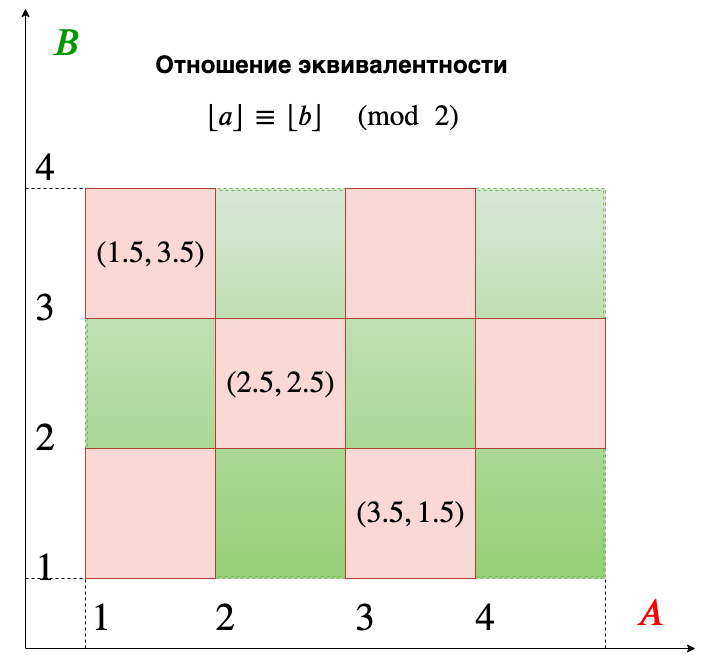
\includegraphics[scale=0.25]{../equiv.png}
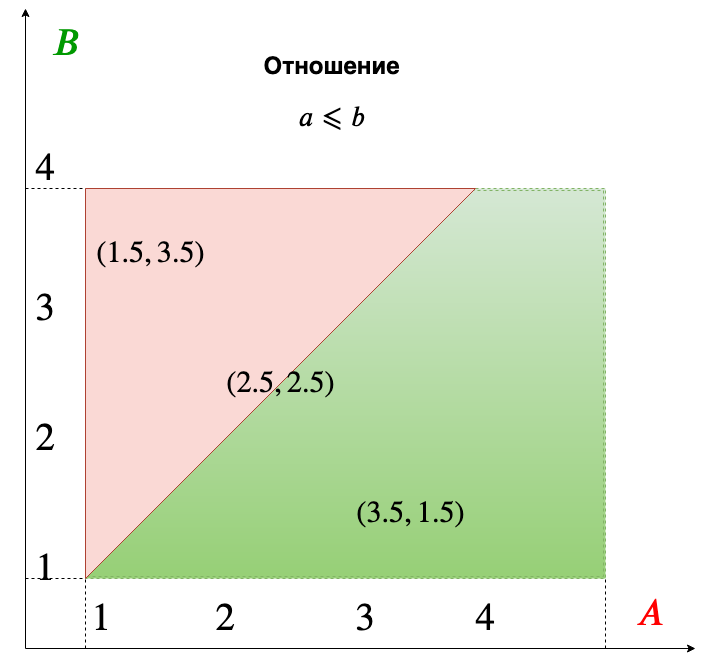
\includegraphics[scale=0.25]{../lessthan.png}
\end{center}

\item *Доказать, что определение упорядоченной пары в виде
$$
(a,b) = \{\{a\},\{a,b\}\}
$$
удовлетворяет требованию \eqref{pairdiff}
\item Рассмотрим соответствие множества людей и множества всех возрастов (целых лет). В каком направлении соответствие между ними является функцией?
\item Рассмотрим соответствие множества людей и банковских счетов. Является ли это соответствие функцией хоть в каком-то направлении?
\item Доказать, что функция $f(x)=3x-7$ биективно отображает $\R$ в $\R$.
\item Доказать, что функция $g(x)=x^2+3x-6$ действует инъективно при $x\in[-3/2,+\infty)$.
\item Докажите, что $F[A\cup C]=F[A]\cup F[C]$ и $F^{-1}[A\cup C]=F^{-1}[A]\cup F^{-1}[C]$.
\item Докажите, что $F[A\cap C]\subseteq F[A]\cap F[C]$ и $F^{-1}[A\cap C]=F^{-1}[A]\cap F^{-1}[C]$.
\item Привести примеры, когда $F[A\cap C]\ne F[A]\cap F[C]$.
\end{enumerate}



\section{Обозначения перестановок}

\subsection*{Справочные сведения}

\subsection*{Задачи}

\begin{enumerate}
\item Пусть $s$ --- некоторая перестановка на $n$ элементах. Для $i,j\in X_n$ запишем $i\sim j$, если существует такое натуральное $k$, что $s^k(i)=j$. Докажите, что
\begin{enumerate}[a)]
\item $\sim$ --- это отношение эквивалентности на множестве $X_n$;
\item классы эквивалентности по данному отношению представляют собой орбиты элементов $X_n$ при действии группы $G(s)$;
\item элементы, входящие в цикл перестановки, составляют класс эквивалентности по отношению $\sim$.
\end{enumerate}
\end{enumerate}



\section{Пара слов о конечных группах}

\subsection*{Справочные сведения}

\subsection*{Задачи}



\section{Знакопеременная группа}

\subsection*{Справочные сведения}

\subsection*{Задачи}




\section{Структура группы перестановок}

\subsection*{Справочные сведения}

\subsection*{Задачи}






\begin{comment}
\chapter{11. Движения плоскости и пространства}
\end{comment}
\newchapter[и пространства]{Движения плоскости}

\section{Виды движений плоскости. Теорема Шаля}

\subsection*{Справочные сведения}

\subsection*{Задачи}


\begin{enumerate}
\item Найти композицию отражения относительно вертикальной оси и поворота на $180^o$ относительно точки, не лежащей на оси симметрии.
\item Пусть дан произвольный треугольник. На его сторонах построим правильные треугольники и соединим их центры. Доказать, что полученный треуголник --- правильный.
\end{enumerate}


\section{Сравнение движений прямой, окружности и плоскости}

\subsection*{Справочные сведения}

\subsection*{Задачи}




\section{Пара слов о движениях сферы}

\subsection*{Справочные сведения}

\subsection*{Задачи}

\begin{enumerate}
\item Построить таблицу движений сферы аналогично таблице движений плоскости (символику придумайте сами).
\item **Доказать, что других движений на сфере не существует (лемма о гвоздях).
\end{enumerate}


\section{Пара слов о движениях пространства}

\subsection*{Справочные сведения}

\subsection*{Задачи}

\begin{enumerate}
\item Построить таблицу движений пространства аналогично таблице движений плоскости (символику придумайте сами).
\item *Показать, что центральная симметрия пространства --- это зеркальное вращение.
\item **Доказать, что других движений в пространстве не существует (лемма о гвоздях).
\end{enumerate}



\begin{comment}
\chapter{12. Комплексная арифметика и алгебра}
\end{comment}
\newchapter[и алгебра]{Комплексная арифметика}


\section{Алгебра комплексных чисел}

\subsection*{Справочные сведения}

\subsection*{Задачи}


\begin{enumerate}
\item Докажите, что если $\la>0$, то $|\la-1|<\la+1$.
\item Вычислить, нарисовать на плоскости и указать модуль и аргумент следующих комплексных чисел:
$$
i^2,\;i^3,\;i^4,\;1/i,\;(1+2i)(2-i),\;(1+i)(1+2i)(1+3i),\;\frac{1}{1+i},\;\frac{5}{2-i}.
$$
\end{enumerate}


\section{Гауссовы целые числа}

\subsection*{Справочные сведения}

\subsection*{Задачи}

\begin{enumerate}
\item Найти все 4 остатка от деления $2+3i$ на $1+i$.
\item Найти минимальный по норме остаток от деления $3+7i$ на $1+2i$.
\end{enumerate}


\begin{comment}
\chapter{13. Введение в линейную алгебру}
\end{comment}
\newchapter[линейную алгебру]{Введение в}\label{linalg}


\section{Преобразования}

\subsection*{Справочные сведения}

\subsection*{Задачи}




\section{Подобия прямой и плоскости}


\subsection*{Справочные сведения}

\subsection*{Задачи}



\section{Линейное пространство}

\subsection*{Справочные сведения}

\subsection*{Задачи}



\section{Линейные операторы}

\subsection*{Справочные сведения}

\subsection*{Задачи}



\section{Арифметика матриц}

\subsection*{Справочные сведения}

\subsection*{Задачи}



\section{Матрицы и комплексные числа}

\subsection*{Справочные сведения}

\subsection*{Задачи}




\section{Действие линейных отображений на векторном пространстве}

\subsection*{Справочные сведения}

\subsection*{Задачи}



\begin{comment}
\chapter{14. Алгебраические числа}
\end{comment}
\newchapter{Алгебраические числа}


\section{*Упорядоченные множества}\label{Ordering}

\subsection*{Справочные сведения}

\subsection*{Задачи}

\begin{enumerate}
\item Пусть множество $X$ не пусто. Верно ли, что $\emptyset<X$? Верно ли, что $X<\emptyset$? Верно ли, что $\emptyset<\emptyset$?
\item Каким отношением (антирефлексивным, транзитивным, связным) является отношение несобственного вложения множеств? $X$ есть несобственное подмножество $Y$ (обозначение: $X\subset Y$), если $X\subseteq Y$ и $X\ne Y$.
\item Каким отношением является отношение делимости $x|y$ на положительных целых числах?
\item Является ли всюду плотным множество всех десятично рациональных чисел, т.е. чисел вида $k/10^n$, где $k\in \Z$ и $n\in\N$?
\item Выпишите полный список аксиом упорядоченного поля.
\end{enumerate}


\section{Плотные множества}

\subsection*{Справочные сведения}

\subsection*{Задачи}



\section{Зазоры между рациональными числами}

\subsection*{Справочные сведения}

\subsection*{Задачи}



\section{О построениях циркулем и линейкой}

\subsection*{Справочные сведения}

\subsection*{Задачи}

\begin{enumerate}
\item Построить циркулем и линейкой отрезки длины $\sqrt 2$ и $\sqrt 3$.
\item Доказать, что $\Q[\sqrt[3]{2}]=\{a+b\sqrt[3]{2}+c\sqrt[3]{4}\;|\;a,b,c\in\Q\}$ и имеет размерность 3 над $\Q$.
\end{enumerate}





\section{Многочлены и алгебраические числа}

\subsection*{Справочные сведения}

\subsection*{Задачи}




\begin{comment}
\chapter{15. Континуум}
\end{comment}
\newchapter{Континуум}


\section{Мощности множеств}\label{powers}

\subsection*{Справочные сведения}

\subsection*{Задачи}

\begin{enumerate}
\item Найти мощность множества всех функций из $X=\{1,2,3\}$ в $Y=\{1,2,3,4\}$.
\item Какова мощность множества $\{(n,m)\mid n,m\in\Z, n<m\}$?
\item Пусть множество $C$ счетное, а множество $X$ бесконечное.
\begin{enumerate}[a)]
\item Доказать, что $X\cup C\leftrightarrow X$ (равномощны).
\item Доказать, что если $X\setminus C$ --- бесконечное, то $X\setminus C\leftrightarrow X$.
\end{enumerate}
\end{enumerate}

\section{Изоморфизмы}

\subsection*{Справочные сведения}

\subsection*{Задачи}


\section{Действительные числа}

\subsection*{Справочные сведения}

\subsection*{Задачи}

\begin{enumerate}
\item Доказать, что между любыми двумя рациональными числами $r\ne q$ лежит какое-то двоично-рациональное.
\end{enumerate}


\section{Модели действительных чисел}

\subsection*{Справочные сведения}

\subsection*{Задачи}

\begin{enumerate}
\item Дать определение вещественного числа $\sqrt[3]{-5}$ с помощью дедекиндового сечения, т.е. построить соответствующую пару подмножеств множества $\Q$.
\end{enumerate}




\begin{comment}
\chapter{16. Элементы математического анализа}
\end{comment}
\newchapter[математического анализа]{Элементы}

\section{Оценки и пределы}

\subsection*{Справочные сведения}

\subsection*{Задачи}


\section{Экспонента}

\subsection*{Справочные сведения}

\subsection*{Задачи}

\begin{enumerate}
\item Пусть дана последовательность
$$
x_n = \left(1+\frac xn\right)^n.
$$
доказать, что она монотонно возрастает и ограничена сверху.
\item А как ведет себя последовательность
$$
y_n = \left(1+\frac xn\right)^{n+1}?
$$
\item Определим логарифм числа $x>0$ по основанию $a>0$ как такое число $y$, что $a^y=x$. Обозначение: $y=\log_a x$. Вывести формулу:
$$
\log_a x = \frac{\ln x}{\ln a} = \frac{\log_b x}{\log_b a}
$$
при любом положительном основании $b$.
\item Сравнить два числа:
$$
5^{\log_7 3}\quad vs\quad   3^{\log_7 5}.
$$

\end{enumerate}



\section{Комплексная экспонента}

\subsection*{Справочные сведения}

\subsection*{Задачи}
\begin{enumerate}
\item Найти решения уравнения $\sin z=4$.
\item Чему равны выражения
$$
\frac{e^{ix}+e^{-ix}}{2},\quad \frac{e^{ix}-e^{-ix}}{2i}?
$$
\end{enumerate}



